\chapter{FUNDAMENTAÇÃO TEÓRICA}

\section{Equações}
\subsection{Tensor Cauchy-Green à direita}
\begin{equation}
    \mathbf{C}=\mathbf{F}^T \mathbf{F}
    \label{eq:cauchyGreen}
\end{equation}
Onde $\mathbf{F}$ é o gradiente de deformação.
Eq. \eqref{eq:cauchyGreen}

\section{Elementos Gráficos}
\subsection{Tabelas}
\begin{table}[H]
    \caption{Descrição da tabela}
    \centering
    \begin{tabular}{c|c}
        A  & B \\
        C & D
    \end{tabular}
    \label{tab:my_label}
\end{table}

\tabela \ref{tab:my_label}

\subsection{Imagens}
\begin{figure}[H]
    \centering
    \caption{Descrição da imagem}
    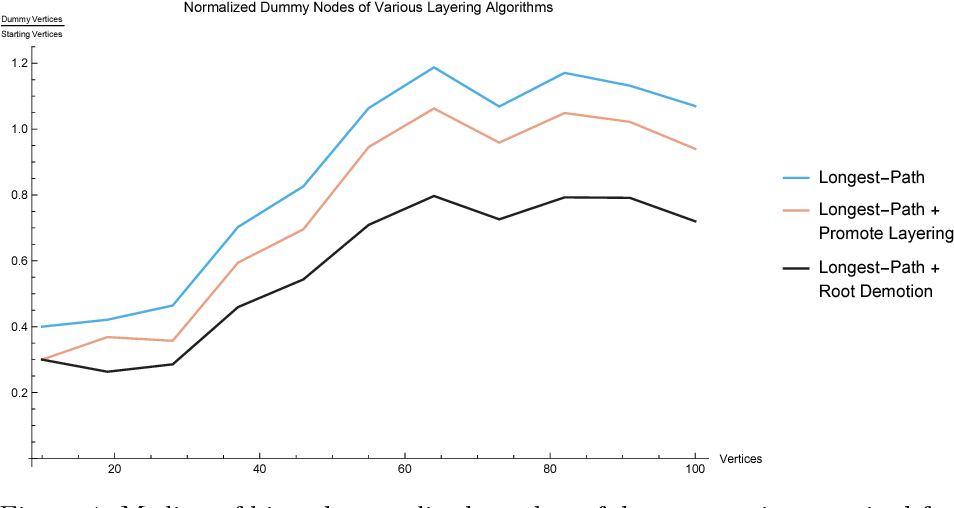
\includegraphics[width=.5\linewidth]{assets/fig.png}
    \label{fig:my_img}
\end{figure}

\section{Citações}
% \cite{Boatti2016AData}
\textcite{Boatti2016AData}
\textcite{Abrahamson2003ShapeResin}

\cite{Abrahamson2003ShapeResin}

\cites{Steven2014ShapeMateriability}{Haupt2002ContinuumMaterials}{Evangelista2010AStrain}

% \section{Otimização dos Parâmetros}
% \subsection{COBYLA}
% \subsection{Distância absoluta média}
% \subsection{Protocolo TCP/IP}

